\documentclass[11pt,a4paper]{article}
\usepackage[margin=2.3cm]{geometry}
\usepackage{booktabs,amsmath,amssymb,microtype,xcolor,caption,float}
\usepackage[hidelinks]{hyperref}
\usepackage{graphicx}
\graphicspath{{figs/}}
\captionsetup{font=small,labelfont=bf}
\setlength{\parskip}{4pt}
\newcommand{\code}[1]{\texttt{\small #1}}

\title{\textbf{MuJoCo CPU vs.\ MuJoCo Warp}\\ Derivative Validation: Experimental Results}
\author{Executed on Unitree Go1, RTX 4090}
\date{\today}
\begin{document}
\maketitle


\begin{abstract}
This document reports the execution of the MuJoCo CPU vs.\ MuJoCo Warp (MJWarp) derivative
validation plan on a floating-base quadruped. All eight phases were run: configuration
freeze, nominal transition parity, CPU black-box finite differences validated against
\code{mjd\_transitionFD}, batched MJWarp finite differences, an epsilon sweep, a directional
Taylor test, contact diagnostics, and wall-time benchmarking. A float64 GPU control (MJX)
was added to separate floating-point precision from GPU batching and from simulator
implementation differences.
The central conclusion is that MJWarp float32 finite differences are accurate and locally
predictive for smooth and stable-contact states over a usable epsilon window roughly two to
three decades coarser than the CPU double-precision optimum; that where they fail --- near
contact-mode switching --- the CPU float64 Jacobian fails identically, so the failure is
contact nonsmoothness rather than precision; and that on a robot of this size the GPU does
not beat a 32-thread CPU rollout pool.
\end{abstract}


\section{Summary of findings}

\begin{enumerate}\itemsep3pt

\item \textbf{The CPU harness is exact.} A manifold-aware black-box central
difference reproduces \code{mjd\_transitionFD} to $1.47\times10^{-16}$ relative Frobenius error over
7 fixtures $\times$ 5 epsilons. Perturbation, output differencing, state packing, control
indexing and warm-start handling are therefore all correct, and every later discrepancy
belongs to the simulator rather than the harness.

\item \textbf{Nominal parity holds.} CPU and MJWarp agree on the unperturbed
one-step map to $\sim$$10^{-7}$ in generalized position, and the contact set is identical
in all 21 fixture$\times$horizon combinations tested ($S \in \{1,5,20\}$).

\item \textbf{A usable epsilon window exists, and it is much wider than the CPU
one.} The MJWarp optimum sits at $h \approx 10^{-3}$--$10^{-4}$ against a CPU optimum of
$10^{-6}$. At the stance fixture the best MJWarp relative error on $A$ is
$4.08\times10^{-4}$ at $h$~=~$10^{-4}$.

\item \textbf{Precision is the limiting factor, not GPU batching.} A float64 GPU
simulator (MJX) on the same card reproduces the CPU Jacobian to $\sim$$10^{-12}$ and shows a
monotone truncation curve with no roundoff turnaround in the swept range. The MJWarp error
curve is U-shaped over the same states and epsilons.

\item \textbf{Where MJWarp fails, CPU float64 fails identically.} In the directional
Taylor test the MJWarp Jacobian predicts the \emph{CPU} simulator as well as the CPU Jacobian
does for stance, sliding and impact. At the near-switching fixtures both have log--log slope
$0.71$ and both plateau at the same residual. That is genuine contact nonsmoothness.

\item \textbf{GPU nondeterminism is a contact phenomenon.} MJWarp is bitwise
reproducible across repeated runs when no contact is active, and nondeterministic as soon as
the constraint solver engages, with run-to-run spread growing like $\eta/h$.

\item \textbf{CUDA graph capture is mandatory.} Launched eagerly, one batched step of
97 worlds costs $\sim$25\,ms of Python kernel-launch overhead; captured into a CUDA graph it
costs $0.37$\,ms. A benchmark run without capture measures the wrong thing by a factor of
20--55.

\item \textbf{A float32 failure that only appears in a batch.} Under the pyramidal
cone the deeply penetrating 8-contact fixture returns NaN in 10 of 97 perturbed worlds; 9 of
those 10 states are finite when re-simulated one world at a time.

\item \textbf{The GPU does not win at this scale.} With graph capture and knot
batching, MJWarp bottoms out at $0.91$\,ms per Jacobian while \code{mujoco.rollout} on 32
threads sustains $0.47$\,ms. MJWarp additionally hits a memory wall well before the GPU is
compute-saturated.

\end{enumerate}

\section{Experimental setup}

The model is \code{unitree\_go1/scene.xml} from MuJoCo Menagerie:
$n_q=19$, $n_v=18$, $n_a=0$, $n_u=12$, giving a tangent state
dimension $n_x = 2n_v + n_a = 36$. A centered difference therefore requires
$2(n_x + n_u) = 96$ perturbed worlds, plus one nominal world for parity
checks. Collision geometry is primitive only (planes, spheres, capsules, boxes, cylinders);
there are no mesh--mesh contacts, which deliberately removes the mesh float32 rounding issue
as a confound.

\begin{table}[htbp]
\centering
\footnotesize
\caption{Software and hardware versions recorded with every result (Phase 0).}
\label{tab:versions}
\begin{tabular}{ll}
\toprule
\textbf{Component} & \textbf{Version} \\
\midrule
MuJoCo (CPU reference and MJWarp runs) & 3.8.1 \\
MJWarp & 3.8.1 \\
NVIDIA Warp & 1.13.0 \\
MuJoCo / JAX (MJX float64 control) & 3.10.0 / 0.6.2 \\
NumPy & 2.4.6 \\
GPU & NVIDIA GeForce RTX 4090, 580.173.02, 8.9 \\
CPU threads available & 32 \\
\bottomrule
\end{tabular}
\end{table}

\subsection{Frozen configuration}
Euler integrator, Newton solver, elliptic friction cone, timestep $2$\,ms, 100 solver
iterations, 50 line-search iterations. One configuration detail is essential and easy to
miss: \textbf{MJWarp silently raises the solver tolerance}. In \code{io.py} it applies
\code{opt.tolerance = max(opt.tolerance, 1e-6)} with the comment that the C MuJoCo tolerance
was chosen for a float64 architecture. If the CPU side is left at its model default of
$10^{-8}$, the two solvers do different amounts of work and nominal parity is confounded
before any derivative is computed. Both sides were therefore pinned to $10^{-6}$.

Warm-start handling mirrors \code{mjd\_transitionFD}: the nominal \code{qacc\_warmstart} is
restored before every perturbed rollout so that all perturbations start the solver
identically, and the same nominal warm start is copied into every MJWarp world.

\begin{table}[htbp]
\centering
\footnotesize
\caption{Representative state suite (Phase 7). \emph{flips} counts how many of the $2n_x$ single-coordinate perturbations at $h=10^{-4}$ change the contact pair set. The two near-switching fixtures were placed at the contact \emph{margin} ($10^{-3}$\,m), which is where the discrete set change occurs, rather than at zero gap.}
\label{tab:fixtures}
\begin{tabular}{llrrrrrl}
\toprule
\textbf{Fixture} & \textbf{Description} & \textbf{ncon} & \textbf{nefc} & \textbf{foot gap [m]} & $\|q_v\|$ & \textbf{flips} & \textbf{difficulty} \\
\midrule
flight & no contact, free fall & 0 & 12 & $5.12\times10^{-1}$ & 0.00 & 0/72 & low \\
stance & 4 contacts, settled & 4 & 36 & $-1.35\times10^{-2}$ & 0.00 & 0/72 & moderate \\
loaded & 8 contacts, pressed down & 8 & 48 & $-3.00\times10^{-2}$ & 0.00 & 0/72 & moderate--high \\
onset & at the contact margin, closing & 1 & 18 & $9.80\times10^{-4}$ & 0.30 & 5/72 & high / nonsmooth \\
release & just outside the margin, opening & 0 & 12 & $1.02\times10^{-3}$ & 0.60 & 1/72 & high / nonsmooth \\
sliding & 4 contacts, 1.2 m/s lateral & 4 & 36 & $-1.35\times10^{-2}$ & 1.20 & 0/72 & high \\
impact & 4 contacts, 3.0 m/s downward & 4 & 36 & $-2.00\times10^{-3}$ & 3.00 & 0/72 & very high \\
\bottomrule
\end{tabular}
\end{table}

\section{Phase 2: the CPU implementation is exact}

Before any GPU comparison can mean anything, the black-box central difference must
reproduce MuJoCo's own staged, stage-skipping \code{mjd\_transitionFD}. It does, at machine
precision: the largest relative Frobenius error over all 7 fixtures and 5 epsilons is
$1.47\times10^{-16}$ for $A$ and $1.47\times10^{-16}$ for $B$
(Table~\ref{tab:phase2}). This validates tangent-space perturbation via
\code{mj\_integratePos}, output differencing via \code{mj\_differentiatePos}, state
packing, actuator-state handling, control indexing and Jacobian layout in one shot.

\begin{table}[htbp]
\centering
\footnotesize
\caption{Phase 2. Relative Frobenius error between the black-box CPU central difference and \code{mjd\_transitionFD} for $A$, as a function of the perturbation size $h$. All values are at double-precision round-off.}
\label{tab:phase2}
\begin{tabular}{lrrrrr}
\toprule
\textbf{Fixture} & $10^{-2}$ & $10^{-3}$ & $10^{-4}$ & $10^{-5}$ & $10^{-6}$ \\
\midrule
flight & $7.4\times10^{-17}$ & $3.5\times10^{-17}$ & $5.2\times10^{-17}$ & $9.8\times10^{-17}$ & $4.9\times10^{-17}$ \\
stance & $3.3\times10^{-17}$ & $6.6\times10^{-17}$ & $4.8\times10^{-17}$ & $1.1\times10^{-16}$ & $1.4\times10^{-16}$ \\
loaded & $8.2\times10^{-17}$ & $3.3\times10^{-17}$ & $1.1\times10^{-16}$ & $1.1\times10^{-16}$ & $1.9\times10^{-17}$ \\
onset & $8.8\times10^{-17}$ & $8.3\times10^{-17}$ & $1.0\times10^{-16}$ & $1.0\times10^{-16}$ & $5.6\times10^{-17}$ \\
release & $8.2\times10^{-17}$ & $5.6\times10^{-17}$ & $9.9\times10^{-17}$ & $1.0\times10^{-16}$ & $2.9\times10^{-17}$ \\
sliding & $5.8\times10^{-17}$ & $5.0\times10^{-17}$ & $4.9\times10^{-17}$ & $3.4\times10^{-17}$ & $7.4\times10^{-17}$ \\
impact & $2.3\times10^{-17}$ & $8.5\times10^{-17}$ & $4.7\times10^{-17}$ & $7.0\times10^{-17}$ & $8.7\times10^{-17}$ \\
\bottomrule
\end{tabular}
\end{table}

\subsection{A warm-start pitfall worth recording}
An early version of the harness computed contact diagnostics by calling \code{mj\_forward}
inside the finite-difference loop. This shifts the resulting Jacobian by $\sim$$10^{-6}$ ---
\emph{even when} \code{qacc\_warmstart} is saved and restored around the diagnostic call.
Contact diagnostics must be collected on a separate \code{MjData} instance that the
finite-difference path never touches. With the diagnostic call in place the agreement with
\code{mjd\_transitionFD} degraded from $10^{-16}$ to $1.4\times10^{-5}$ on the impact
fixture; with it removed, agreement is exact.

\section{Phase 1: nominal transition parity}

\begin{table}[htbp]
\centering
\footnotesize
\caption{Phase 1. Manifold-aware distance between the CPU and MJWarp unperturbed next state. Position error sits at the float32 floor; the contact pair set is identical everywhere. There is no physics or collision disagreement to confound the derivative comparison.}
\label{tab:phase1}
\begin{tabular}{lrrrrcc}
\toprule
\textbf{Fixture} & $\|\Delta q\|_{\mathrm{tan}}$ ($S{=}1$) & $\|\Delta v\|$ ($S{=}1$) & $\|\Delta q\|$ ($S{=}20$) & $\|\Delta v\|$ ($S{=}20$) & \textbf{ncon C/W} & \textbf{pairs} \\
\midrule
flight & $1.11\times10^{-7}$ & $1.24\times10^{-7}$ & $1.27\times10^{-7}$ & $7.12\times10^{-7}$ & 0/0 & match \\
stance & $9.53\times10^{-8}$ & $3.77\times10^{-7}$ & $1.02\times10^{-7}$ & $1.78\times10^{-6}$ & 4/4 & match \\
loaded & $2.35\times10^{-7}$ & $1.02\times10^{-4}$ & $6.41\times10^{-6}$ & $1.01\times10^{-4}$ & 8/8 & match \\
onset & $9.90\times10^{-8}$ & $1.43\times10^{-6}$ & $3.16\times10^{-7}$ & $5.30\times10^{-6}$ & 2/2 & match \\
release & $1.46\times10^{-7}$ & $1.91\times10^{-6}$ & $2.11\times10^{-7}$ & $6.51\times10^{-6}$ & 0/0 & match \\
sliding & $1.45\times10^{-7}$ & $2.30\times10^{-6}$ & $2.19\times10^{-7}$ & $9.27\times10^{-6}$ & 4/4 & match \\
impact & $1.26\times10^{-7}$ & $6.29\times10^{-6}$ & $3.11\times10^{-5}$ & $5.39\times10^{-4}$ & 4/4 & match \\
\bottomrule
\end{tabular}
\end{table}

\section{Phases 3--4: batched MJWarp finite differences and the epsilon sweep}

Worlds are laid out as
$[x{+}0,\,x{-}0,\,x{+}1,\,x{-}1,\dots,u{+}0,u{-}0,\dots]$ with a nominal world appended.
Generalized-position perturbations are built on the host in float64 with
\code{mj\_integratePos}, uploaded as float32, and the returned states are up-cast to float64
before differencing with \code{mj\_differentiatePos}, so the only float32 in the pipeline is
the simulation itself.

Three error curves are reported per fixture, all against $A_{\mathrm{gold}}$ = CPU float64 at
$h=10^{-6}$:
\begin{align*}
E_{\mathrm{same}}(h) &= \|A_{\mathrm{warp}}(h) - A_{\mathrm{cpu}}(h)\|_F / \|A_{\mathrm{cpu}}(h)\|_F
 &&\text{GPU vs.\ CPU at matched truncation}\\
E_{\mathrm{gold}}(h) &= \|A_{\mathrm{warp}}(h) - A_{\mathrm{gold}}\|_F / \|A_{\mathrm{gold}}\|_F
 &&\text{total error of the GPU Jacobian}\\
E_{\mathrm{cpu}}(h)  &= \|A_{\mathrm{cpu}}(h) - A_{\mathrm{gold}}\|_F / \|A_{\mathrm{gold}}\|_F
 &&\text{the CPU's own truncation curve}
\end{align*}
Separating these is what makes the results interpretable: at large $h$, $E_{\mathrm{same}}$ is
orders of magnitude smaller than $E_{\mathrm{gold}}$, which says the large-$h$ error is shared
truncation and not a GPU defect.

\begin{figure}[htbp]\centering
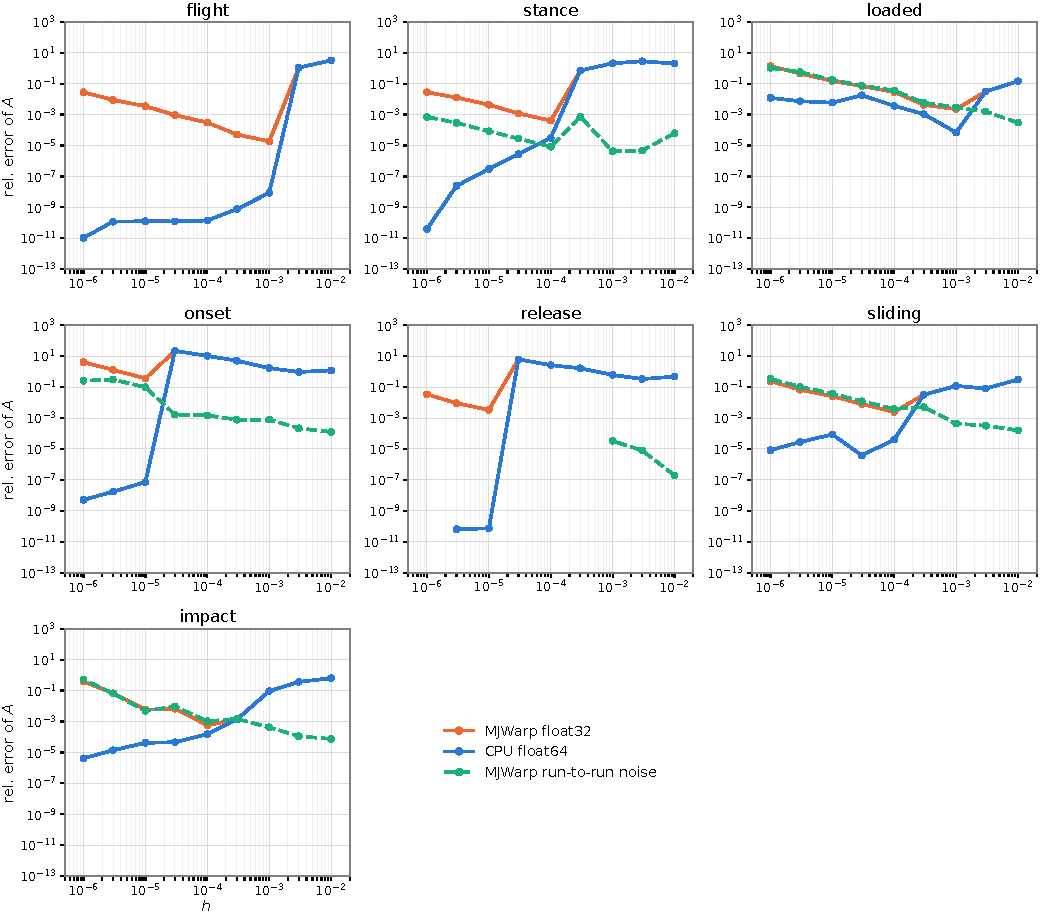
\includegraphics[width=\linewidth]{sweep.pdf}
\caption{Phase 4 epsilon sweep, elliptic cone, $S=1$. The MJWarp curve (orange) is U-shaped:
truncation on the right, float32 cancellation and nondeterminism on the left. The CPU curve
(blue) keeps falling. For \code{onset} and \code{release} the two coincide over the
contact-switching region, which is the signature of nonsmoothness rather than precision.
The dashed line is MJWarp's run-to-run spread, which is identically zero for \code{flight}
and therefore absent from that panel.}
\label{fig:sweep}\end{figure}

\begin{table}[htbp]
\centering
\footnotesize
\caption{Phase 4, elliptic cone, $S=1$. The MJWarp optimum lies two to three decades coarser than the CPU optimum. Column cosine is the minimum over columns whose reference norm is meaningful.}
\label{tab:besteps}
\begin{tabular}{lrrrrrrr}
\toprule
\textbf{Fixture} & \textbf{best }$h$ & $E_{\mathrm{gold}}(A)$ & $E_{\mathrm{gold}}(B)$ & \textbf{min col.\ cos} & \textbf{GPU noise} & \textbf{best }$h$\textbf{ CPU} & $E_{\mathrm{cpu}}$ \\
\midrule
flight & $10^{-3}$ & $1.86\times10^{-5}$ & $2.73\times10^{-5}$ & 1.0000 & $0$ & $10^{-6}$ & $1.07\times10^{-11}$ \\
stance & $10^{-4}$ & $4.08\times10^{-4}$ & $8.89\times10^{-4}$ & 1.0000 & $8.32\times10^{-6}$ & $10^{-6}$ & $3.97\times10^{-11}$ \\
loaded & $10^{-3}$ & $2.23\times10^{-3}$ & $3.12\times10^{-3}$ & 0.9998 & $2.91\times10^{-3}$ & $10^{-3}$ & $6.95\times10^{-5}$ \\
onset & $10^{-5}$ & $3.66\times10^{-1}$ & $2.48\times10^{-1}$ & -0.6366 & $9.78\times10^{-2}$ & $10^{-6}$ & $5.06\times10^{-9}$ \\
release & $10^{-5}$ & $3.38\times10^{-3}$ & $3.18\times10^{-3}$ & 0.9999 & $0$ & $10^{-6}$ & $0$ \\
sliding & $10^{-4}$ & $2.44\times10^{-3}$ & $1.65\times10^{-2}$ & 0.9878 & $3.92\times10^{-3}$ & $3\times10^{-5}$ & $3.80\times10^{-6}$ \\
impact & $10^{-4}$ & $5.78\times10^{-4}$ & $1.55\times10^{-3}$ & 0.9996 & $1.04\times10^{-3}$ & $10^{-6}$ & $4.16\times10^{-6}$ \\
\bottomrule
\end{tabular}
\end{table}

\begin{table}[htbp]
\centering
\footnotesize
\caption{Full epsilon sweep for the \code{stance} fixture, elliptic cone, $S=1$. The clean U-shape of a contact-stable state: $E_{\mathrm{same}}$ stays small throughout, so MJWarp tracks the CPU at matched $h$; the total error is truncation-dominated above $10^{-4}$ and noise-dominated below.}
\label{tab:sweepstance}
\begin{tabular}{lrrrrrcrr}
\toprule
$h$ & $E_{\mathrm{same}}$ & $E_{\mathrm{gold}}$ & $E_{\mathrm{cpu}}$ & \textbf{noise} & \textbf{cos} & \textbf{stable} & $E$\textbf{ stable} & $E$\textbf{ changing} \\
\midrule
$10^{-2}$ & $4.68\times10^{-5}$ & $2.00\times10^{0}$ & $2.00\times10^{0}$ & $6.27\times10^{-5}$ & 0.8503 & 35/36 & $2.44\times10^{0}$ & $1.91\times10^{0}$ \\
$3\times10^{-3}$ & $8.80\times10^{-5}$ & $2.79\times10^{0}$ & $2.79\times10^{0}$ & $4.72\times10^{-6}$ & 0.8965 & 36/36 & $2.79\times10^{0}$ & --- \\
$10^{-3}$ & $2.23\times10^{-5}$ & $2.07\times10^{0}$ & $2.07\times10^{0}$ & $4.24\times10^{-6}$ & 0.9419 & 36/36 & $2.07\times10^{0}$ & --- \\
$3\times10^{-4}$ & $1.48\times10^{-3}$ & $7.03\times10^{-1}$ & $7.04\times10^{-1}$ & $7.25\times10^{-4}$ & 0.9946 & 36/36 & $7.03\times10^{-1}$ & --- \\
$10^{-4}$ & $4.07\times10^{-4}$ & $4.08\times10^{-4}$ & $3.06\times10^{-5}$ & $8.32\times10^{-6}$ & 1.0000 & 36/36 & $4.08\times10^{-4}$ & --- \\
$3\times10^{-5}$ & $1.18\times10^{-3}$ & $1.18\times10^{-3}$ & $2.75\times10^{-6}$ & $2.77\times10^{-5}$ & 0.9998 & 36/36 & $1.18\times10^{-3}$ & --- \\
$10^{-5}$ & $4.35\times10^{-3}$ & $4.35\times10^{-3}$ & $3.03\times10^{-7}$ & $8.37\times10^{-5}$ & 0.9960 & 36/36 & $4.35\times10^{-3}$ & --- \\
$3\times10^{-6}$ & $1.25\times10^{-2}$ & $1.25\times10^{-2}$ & $2.45\times10^{-8}$ & $2.88\times10^{-4}$ & 0.9682 & 36/36 & $1.25\times10^{-2}$ & --- \\
$10^{-6}$ & $2.79\times10^{-2}$ & $2.79\times10^{-2}$ & $3.97\times10^{-11}$ & $7.06\times10^{-4}$ & 0.9564 & 36/36 & $2.79\times10^{-2}$ & --- \\
\bottomrule
\end{tabular}
\end{table}

\begin{table}[htbp]
\centering
\footnotesize
\caption{Full epsilon sweep for the \code{onset} fixture, elliptic cone, $S=1$. A near-switching state. $E_{\mathrm{gold}}$ and $E_{\mathrm{cpu}}$ are \emph{identical} for $h\geq3\times10^{-5}$ --- the error is entirely shared nonsmoothness. Only when perturbations stop crossing the contact boundary (36/36 stable columns) does the CPU error collapse, at which point float32 noise dominates the GPU.}
\label{tab:sweeponset}
\begin{tabular}{lrrrrrcrr}
\toprule
$h$ & $E_{\mathrm{same}}$ & $E_{\mathrm{gold}}$ & $E_{\mathrm{cpu}}$ & \textbf{noise} & \textbf{cos} & \textbf{stable} & $E$\textbf{ stable} & $E$\textbf{ changing} \\
\midrule
$10^{-2}$ & $1.95\times10^{-4}$ & $1.20\times10^{0}$ & $1.20\times10^{0}$ & $1.27\times10^{-4}$ & 0.1540 & 22/36 & $3.73\times10^{-3}$ & $1.27\times10^{0}$ \\
$3\times10^{-3}$ & $9.25\times10^{-4}$ & $9.51\times10^{-1}$ & $9.51\times10^{-1}$ & $2.18\times10^{-4}$ & 0.1297 & 25/36 & $2.38\times10^{-3}$ & $1.12\times10^{0}$ \\
$10^{-3}$ & $2.18\times10^{-3}$ & $1.70\times10^{0}$ & $1.70\times10^{0}$ & $7.85\times10^{-4}$ & 0.0676 & 28/36 & $9.88\times10^{-2}$ & $2.56\times10^{0}$ \\
$3\times10^{-4}$ & $2.60\times10^{-3}$ & $5.07\times10^{0}$ & $5.07\times10^{0}$ & $7.82\times10^{-4}$ & 0.0349 & 29/36 & $1.67\times10^{-2}$ & $8.19\times10^{0}$ \\
$10^{-4}$ & $4.08\times10^{-3}$ & $1.05\times10^{1}$ & $1.05\times10^{1}$ & $1.49\times10^{-3}$ & 0.0064 & 32/36 & $4.28\times10^{-2}$ & $3.09\times10^{1}$ \\
$3\times10^{-5}$ & $5.82\times10^{-3}$ & $2.21\times10^{1}$ & $2.21\times10^{1}$ & $1.66\times10^{-3}$ & 0.1598 & 35/36 & $1.29\times10^{-1}$ & $6.92\times10^{2}$ \\
$10^{-5}$ & $3.66\times10^{-1}$ & $3.66\times10^{-1}$ & $7.21\times10^{-8}$ & $9.78\times10^{-2}$ & -0.6366 & 36/36 & $3.66\times10^{-1}$ & --- \\
$3\times10^{-6}$ & $1.31\times10^{0}$ & $1.31\times10^{0}$ & $1.73\times10^{-8}$ & $3.10\times10^{-1}$ & -0.1961 & 36/36 & $1.31\times10^{0}$ & --- \\
$10^{-6}$ & $4.09\times10^{0}$ & $4.09\times10^{0}$ & $5.06\times10^{-9}$ & $2.59\times10^{-1}$ & -0.7833 & 36/36 & $4.09\times10^{0}$ & --- \\
\bottomrule
\end{tabular}
\end{table}

\begin{table}[htbp]
\centering
\footnotesize
\caption{Direct differentiation of the full $S$-substep shooting map $F_H = f^S$, rather than chaining substep Jacobians. The optimum epsilon is stable across horizon length and the achievable accuracy does not collapse; the near-switching fixtures actually improve at $S=5$ because the contact mode settles within the interval.}
\label{tab:substep}
\begin{tabular}{lrrrrrr}
\toprule
\textbf{Fixture} & $h^\ast$ ($S{=}1$) & $E_{\mathrm{gold}}$ & $h^\ast$ ($S{=}5$) & $E_{\mathrm{gold}}$ & $h^\ast$ ($S{=}20$) & $E_{\mathrm{gold}}$ \\
\midrule
flight & $10^{-3}$ & $1.9\times10^{-5}$ & $10^{-3}$ & $4.8\times10^{-5}$ & $10^{-3}$ & $2.1\times10^{-4}$ \\
stance & $10^{-4}$ & $4.1\times10^{-4}$ & $10^{-4}$ & $6.5\times10^{-4}$ & $10^{-4}$ & $1.9\times10^{-2}$ \\
loaded & $10^{-3}$ & $2.2\times10^{-3}$ & $3\times10^{-4}$ & $1.4\times10^{-3}$ & $3\times10^{-4}$ & $10.0\times10^{-3}$ \\
onset & $10^{-5}$ & $3.7\times10^{-1}$ & $10^{-5}$ & $8.1\times10^{-2}$ & $3\times10^{-3}$ & $1.8\times10^{-1}$ \\
release & $10^{-5}$ & $3.4\times10^{-3}$ & $10^{-5}$ & $9.8\times10^{-3}$ & $10^{-5}$ & $3.6\times10^{-2}$ \\
sliding & $10^{-4}$ & $2.4\times10^{-3}$ & $10^{-4}$ & $6.6\times10^{-3}$ & $10^{-4}$ & $7.5\times10^{-3}$ \\
impact & $10^{-4}$ & $5.8\times10^{-4}$ & $3\times10^{-4}$ & $3.6\times10^{-3}$ & $3\times10^{-4}$ & $8.4\times10^{-3}$ \\
\bottomrule
\end{tabular}
\end{table}

\section{Precision control: CPU float64 vs.\ MJX float64 vs.\ MJWarp float32}

The epsilon sweep alone cannot separate three candidate causes of MJWarp error:
float32 precision, GPU nondeterminism, and a physics or collision implementation difference.
A float64 GPU simulator settles it. MJX runs the same MuJoCo model on the same RTX 4090 in
double precision under \code{jax\_enable\_x64}; verified on a single step, it reproduces the
CPU next state to $2.3\times10^{-18}$.

MJX does not implement the elliptic friction cone for \code{condim=1}, so this comparison was
re-run for all three simulators with the \textbf{pyramidal} cone. The gold Jacobian norms
agree to four significant figures across the two stacks
($\|A_{\mathrm{gold}}\|_F$: 10.72, 24.94, 82.72, 260.2 for stance, onset, sliding, impact),
confirming the configurations are matched.

\begin{figure}[htbp]\centering
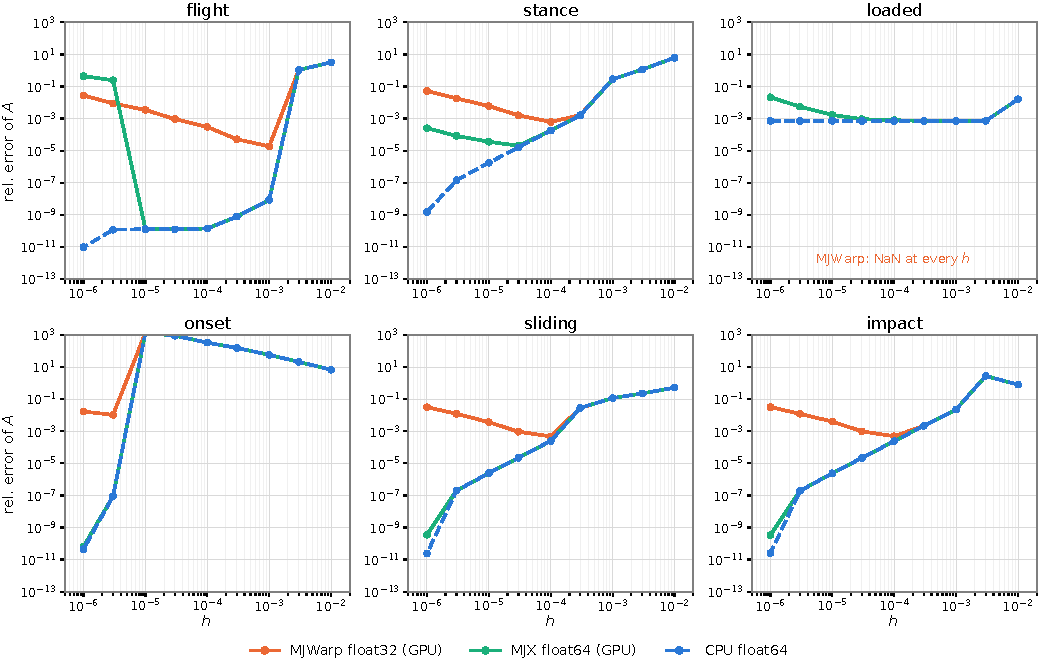
\includegraphics[width=\linewidth]{precision.pdf}
\caption{Precision isolated. Same model, same options (pyramidal cone), same GPU, identical
perturbations. MJX float64 (green) tracks the CPU curve (blue, dashed); MJWarp float32
(orange) turns around near $h\approx10^{-3}$. The \code{loaded} panel has no MJWarp curve
because MJWarp returns NaN at every epsilon for that fixture (Section~\ref{sec:nan}).}
\label{fig:precision}\end{figure}

\begin{table}[htbp]
\centering
\footnotesize
\caption{Best achievable relative error on $A$ and run-to-run spread, GPU float64 vs.\ GPU float32, pyramidal cone. The float64 GPU is three to seven orders of magnitude better on both axes, which attributes the MJWarp limitation to precision rather than to batching or physics.}
\label{tab:precision}
\begin{tabular}{lrrrrrr}
\toprule
\textbf{Fixture} & $h^\ast$ & \textbf{MJX64 err} & \textbf{MJX64 noise} & $h^\ast$ & \textbf{MJWarp32 err} & \textbf{MJWarp32 noise} \\
\midrule
flight & $3\times10^{-5}$ & $1.24\times10^{-10}$ & $1.33\times10^{-13}$ & $10^{-3}$ & $1.86\times10^{-5}$ & $0$ \\
stance & $3\times10^{-5}$ & $2.02\times10^{-5}$ & $3.16\times10^{-6}$ & $10^{-4}$ & $6.16\times10^{-4}$ & $3.86\times10^{-4}$ \\
loaded & $10^{-3}$ & $7.14\times10^{-4}$ & $1.25\times10^{-5}$ & --- & NaN & NaN \\
onset & $10^{-6}$ & $6.44\times10^{-11}$ & $2.31\times10^{-11}$ & $3\times10^{-6}$ & $1.06\times10^{-2}$ & $1.60\times10^{-3}$ \\
sliding & $10^{-6}$ & $3.58\times10^{-10}$ & $1.45\times10^{-11}$ & $10^{-4}$ & $4.83\times10^{-4}$ & $7.11\times10^{-5}$ \\
impact & $10^{-6}$ & $3.40\times10^{-10}$ & $1.04\times10^{-11}$ & $10^{-4}$ & $4.88\times10^{-4}$ & $6.55\times10^{-5}$ \\
\bottomrule
\end{tabular}
\end{table}

\subsection{Run-to-run nondeterminism}
Repeated evaluations with bitwise-identical inputs quantify GPU nondeterminism. The result
has a clean structure: \textbf{MJWarp is bitwise reproducible when no contact is active} ---
the flight fixture returns exactly zero spread across five runs at every epsilon --- and
becomes nondeterministic as soon as the constraint solver engages. The spread then grows as
$h$ shrinks, consistent with the predicted $O(\eta/h)$ amplification of simulator output
noise $\eta$.

\begin{table}[htbp]
\centering
\footnotesize
\caption{MJWarp run-to-run spread of $A$ (maximum pairwise relative Frobenius difference over 5 identical evaluations), elliptic cone, $S=1$. Zero means bitwise identical.}
\label{tab:noise}
\begin{tabular}{lrrrrr}
\toprule
\textbf{Fixture} & $10^{-2}$ & $10^{-3}$ & $10^{-4}$ & $10^{-5}$ & $10^{-6}$ \\
\midrule
flight & $0$ & $0$ & $0$ & $0$ & $0$ \\
stance & $6.3\times10^{-5}$ & $4.2\times10^{-6}$ & $8.3\times10^{-6}$ & $8.4\times10^{-5}$ & $7.1\times10^{-4}$ \\
loaded & $3.0\times10^{-4}$ & $2.9\times10^{-3}$ & $3.6\times10^{-2}$ & $1.7\times10^{-1}$ & $1.0\times10^{0}$ \\
onset & $1.3\times10^{-4}$ & $7.9\times10^{-4}$ & $1.5\times10^{-3}$ & $9.8\times10^{-2}$ & $2.6\times10^{-1}$ \\
release & $1.9\times10^{-7}$ & $3.3\times10^{-5}$ & $0$ & $0$ & $0$ \\
sliding & $1.6\times10^{-4}$ & $4.4\times10^{-4}$ & $3.9\times10^{-3}$ & $3.8\times10^{-2}$ & $3.4\times10^{-1}$ \\
impact & $7.5\times10^{-5}$ & $4.2\times10^{-4}$ & $1.0\times10^{-3}$ & $4.8\times10^{-3}$ & $5.2\times10^{-1}$ \\
\bottomrule
\end{tabular}
\end{table}

\section{Phase 6: contact diagnostics}

The plan warns that folding contact-stable and contact-changing perturbations into a
single Frobenius norm hides the actual behaviour. The data confirm it emphatically. Every
perturbed rollout is checked for whether the $+h$ and $-h$ states preserved the nominal
contact pair set, and the error is reported separately over the two column groups.

\begin{table}[htbp]
\centering
\footnotesize
\caption{The \code{onset} fixture, elliptic cone. At $h=10^{-4}$ the 32 contact-stable columns carry a relative error of $4.3\times10^{-2}$ while the 4 contact-changing columns carry $3.1\times10^{1}$ --- nearly three orders of magnitude apart, averaged into one uninformative number if reported together. As $h$ shrinks the perturbations stop crossing the contact margin and the column count returns to 36/36.}
\label{tab:split}
\begin{tabular}{lcrrr}
\toprule
$h$ & \textbf{stable cols} & $E$ \textbf{contact-stable} & $E$ \textbf{contact-changing} & $E$ \textbf{combined} \\
\midrule
$10^{-2}$ & 22/36 & $3.73\times10^{-3}$ & $1.27\times10^{0}$ & $1.20\times10^{0}$ \\
$3\times10^{-3}$ & 25/36 & $2.38\times10^{-3}$ & $1.12\times10^{0}$ & $9.51\times10^{-1}$ \\
$10^{-3}$ & 28/36 & $9.88\times10^{-2}$ & $2.56\times10^{0}$ & $1.70\times10^{0}$ \\
$3\times10^{-4}$ & 29/36 & $1.67\times10^{-2}$ & $8.19\times10^{0}$ & $5.07\times10^{0}$ \\
$10^{-4}$ & 32/36 & $4.28\times10^{-2}$ & $3.09\times10^{1}$ & $1.05\times10^{1}$ \\
$3\times10^{-5}$ & 35/36 & $1.29\times10^{-1}$ & $6.92\times10^{2}$ & $2.21\times10^{1}$ \\
$10^{-5}$ & 36/36 & $3.66\times10^{-1}$ & --- (none) & $3.66\times10^{-1}$ \\
$3\times10^{-6}$ & 36/36 & $1.31\times10^{0}$ & --- (none) & $1.31\times10^{0}$ \\
$10^{-6}$ & 36/36 & $4.09\times10^{0}$ & --- (none) & $4.09\times10^{0}$ \\
\bottomrule
\end{tabular}
\end{table}

\section{Phase 5: directional Taylor test}

Matrix agreement is a proxy. What a trajectory optimizer actually needs is that the
Jacobian predicts the local behaviour of the simulator. For random tangent directions
$\delta x, \delta u$ the residual
\[
r(\alpha) = d_x\!\left(F(x \oplus \alpha\,\delta x,\; u + \alpha\,\delta u),\;
F(x,u) \oplus \alpha\,(A\,\delta x + B\,\delta u)\right)
\]
should decrease approximately quadratically away from nonsmooth transitions. Three variants
were run: CPU Jacobian against CPU rollouts (the best achievable), MJWarp Jacobian against
MJWarp rollouts (self-consistency), and --- the one that matters --- \textbf{MJWarp Jacobian
against CPU rollouts}, which asks whether the float32 GPU Jacobian predicts the true
double-precision simulator.

\begin{figure}[htbp]\centering
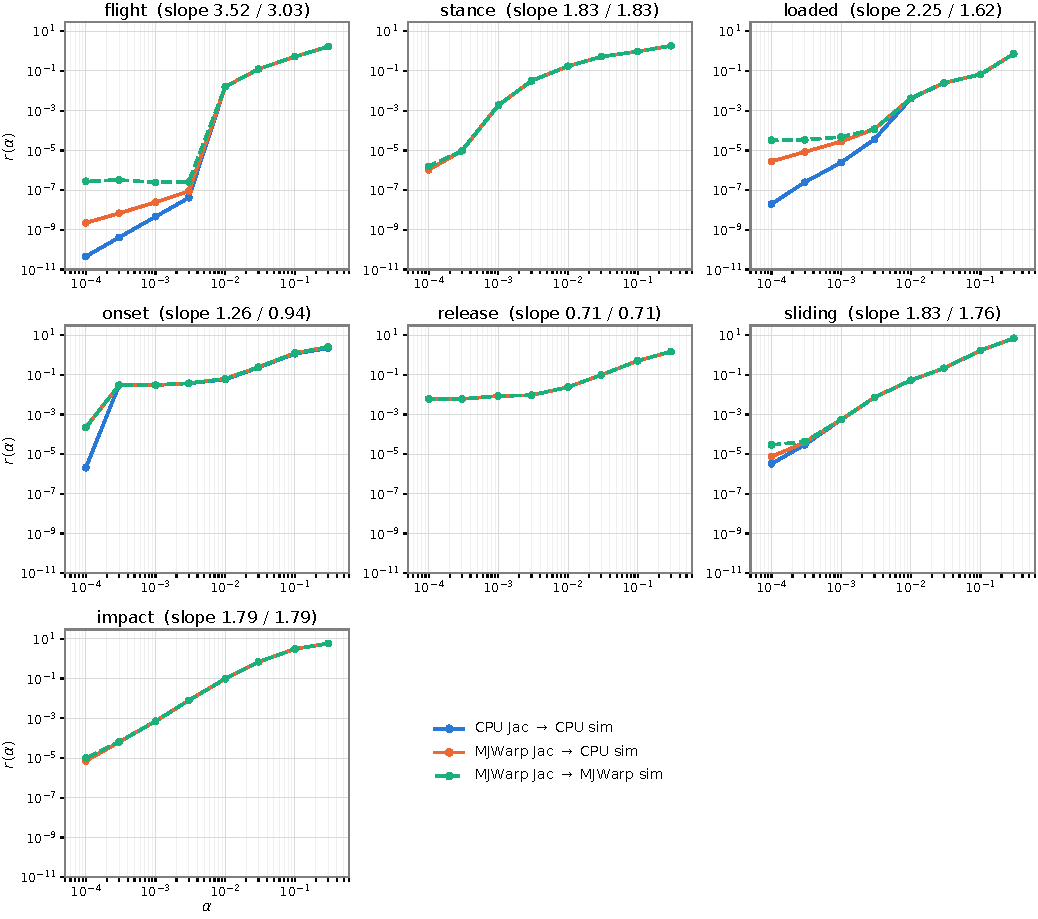
\includegraphics[width=\linewidth]{taylor.pdf}
\caption{Directional Taylor residual, median over 4 random directions, $S=1$. Panel titles give
the log--log slopes (CPU$\to$CPU / MJWarp$\to$CPU). For stance, sliding and impact the orange
curve lies on top of the blue one: the float32 GPU Jacobian predicts the double-precision
simulator as accurately as the CPU Jacobian does. At \code{release} both plateau at
$6\times10^{-3}$ with slope $0.71$ --- the CPU Jacobian is equally non-predictive there.}
\label{fig:taylor}\end{figure}

\begin{table}[htbp]
\centering
\footnotesize
\caption{Log--log slopes of the Taylor residual and the residual at the smallest step. A slope near 2 indicates a valid first-order model. Contact states sit near 1.8 even on the CPU; the two near-switching fixtures fall to 1.26 and 0.71 \emph{identically} for CPU and MJWarp.}
\label{tab:taylor}
\begin{tabular}{lrrrrrr}
\toprule
\textbf{Fixture} & $h$ \textbf{(Warp)} & \textbf{slope} C$\to$C & \textbf{slope} W$\to$C & \textbf{slope} W$\to$W & $r$ \textbf{at} $\alpha{=}10^{-4}$ C$\to$C & $r$ \textbf{at} $\alpha{=}10^{-4}$ W$\to$C \\
\midrule
flight & $10^{-3}$ & 3.52 & 3.03 & 2.40 & $4.6\times10^{-11}$ & $2.2\times10^{-9}$ \\
stance & $10^{-4}$ & 1.83 & 1.83 & 1.80 & $1.1\times10^{-6}$ & $1.0\times10^{-6}$ \\
loaded & $10^{-3}$ & 2.25 & 1.62 & 1.35 & $2.0\times10^{-8}$ & $2.8\times10^{-6}$ \\
onset & $10^{-5}$ & 1.26 & 0.94 & 0.94 & $2.1\times10^{-6}$ & $2.2\times10^{-4}$ \\
release & $10^{-5}$ & 0.71 & 0.71 & 0.71 & $6.0\times10^{-3}$ & $6.0\times10^{-3}$ \\
sliding & $10^{-4}$ & 1.83 & 1.76 & 1.65 & $3.3\times10^{-6}$ & $7.5\times10^{-6}$ \\
impact & $10^{-4}$ & 1.79 & 1.79 & 1.76 & $7.1\times10^{-6}$ & $7.1\times10^{-6}$ \\
\bottomrule
\end{tabular}
\end{table}

\section{Robustness: a float32 failure that only appears in a batch}

\label{sec:nan}

Under the pyramidal cone, the \code{loaded} fixture --- 8 contacts, 3\,cm
penetration, 68 active constraints --- makes MJWarp return NaN in 10 of the 97
perturbed worlds, poisoning 8 columns of $A$ and therefore the whole Jacobian, at every
epsilon in the sweep. The nominal unperturbed step is finite and matches the CPU
($\max|q_v| = 0.6638$ vs.\ $0.6638$), and both CPU float64 and MJX float64 handle every one
of the offending states without difficulty.

The diagnostic detail that matters: re-simulating those same states \textbf{one world at a
time}, 9 of the 10 come back finite. Re-batching the same 10
states as a 10-world problem reproduces the NaN. Whether the float32 Newton solve diverges
therefore depends on the batch in which it is evaluated --- a consequence of the same
reduction-ordering nondeterminism measured in Table~\ref{tab:noise}, acting on a solve that
is marginal in single precision. This class of failure will not reproduce in a single-world
debug session.

\begin{table}[htbp]
\centering
\footnotesize
\caption{The 10 worlds that return NaN inside the 97-world batch (pyramidal cone, \code{loaded}, $h=10^{-3}$). Nine of them are finite when simulated in isolation. The elliptic-cone configuration of the same fixture never exhibits this.}
\label{tab:nan}
\begin{tabular}{lcc}
\toprule
\textbf{World index} & \textbf{Re-run alone} & \textbf{CPU} $\max|q_v|$ \\
\midrule
14 & finite & 0.6637--0.6644 \\
26 & \textbf{NaN} & 0.6637--0.6644 \\
44 & finite & 0.6637--0.6644 \\
47 & finite & 0.6637--0.6644 \\
52 & finite & 0.6637--0.6644 \\
61 & finite & 0.6637--0.6644 \\
66 & finite & 0.6637--0.6644 \\
67 & finite & 0.6637--0.6644 \\
77 & finite & 0.6637--0.6644 \\
89 & finite & 0.6637--0.6644 \\
\bottomrule
\end{tabular}
\end{table}

\textbf{Practical consequence:} validate \code{isfinite} on every returned world
before assembling $A$ and $B$, and treat a NaN world as a failed column rather than letting
it propagate silently into the optimizer.

\section{Wall time and scaling}

\subsection{CUDA graph capture is not optional}
MJWarp issues many small kernels per step. Launched eagerly from Python, a single batched
step of 97 go1 worlds is dominated by launch overhead. Captured into a CUDA graph it is 20 to
55 times faster, and MJWarp's \code{graph\_conditional} option (which uses CUDA conditional
graph nodes for the data-dependent solver iteration count) is worth a further factor of
$\sim$8.

\begin{table}[htbp]
\centering
\footnotesize
\caption{One batched MJWarp step, 97 go1 worlds. Oversized constraint arrays also cost time, not just memory.}
\label{tab:graphmode}
\begin{tabular}{rrlrr}
\toprule
\code{nconmax} & \code{njmax} & \code{graph\_conditional} & \textbf{eager [ms]} & \textbf{captured [ms]} \\
\midrule
6208 & 49664 & on & 56.84 & 0.52 \\
1552 & 6208 & on & 15.64 & 0.34 \\
1552 & 6208 & off & 31.34 & 2.93 \\
\bottomrule
\end{tabular}
\end{table}

\begin{table}[htbp]
\centering
\footnotesize
\caption{Wall time in milliseconds for one $(A,B)$ pair, 97 worlds, $h=10^{-4}$, median of 30 repetitions. \code{mjd\_transitionFD} is one-step only. \emph{GPU only} excludes host-side perturbation construction, download and Jacobian assembly. The threaded CPU finite difference was verified to agree with the serial one to $3.3\times10^{-13}$.}
\label{tab:bench}
\begin{tabular}{lrrrrrrr}
\toprule
\textbf{Horizon} & \code{mjd\_transitionFD} & \textbf{CPU serial} & \textbf{CPU 32 thr} & \textbf{Warp eager} & \textbf{Warp graph} & \textbf{GPU only} & \textbf{vs 32 thr} \\
\midrule
$S=1$ & 0.80 & 2.09 & 1.15 & 25.38 & 1.26 & 0.37 & 0.91$\times$ \\
$S=5$ & --- & 7.81 & 1.41 & 115.40 & 2.49 & 1.60 & 0.57$\times$ \\
$S=20$ & --- & 28.95 & 2.95 & 458.13 & 8.40 & 7.51 & 0.35$\times$ \\
\bottomrule
\end{tabular}
\end{table}

\begin{figure}[htbp]\centering
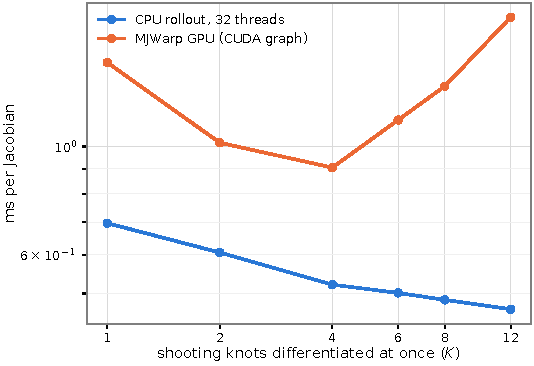
\includegraphics[width=0.62\linewidth]{scale.pdf}
\caption{Cost per Jacobian as a function of the number of shooting knots differentiated
simultaneously. Both sides receive one batched dispatch of $K\times96$ rollouts. The GPU
amortizes to a minimum at $K=4$ and then degrades; the CPU is flat to slightly improving.}
\label{fig:scale}\end{figure}

\begin{table}[htbp]
\centering
\footnotesize
\caption{Cost per Jacobian when $K$ shooting knots are differentiated simultaneously, $S=5$. Both sides receive one batched dispatch of $K\times96$ rollouts: a single CUDA-graph launch on the GPU, a single \code{mujoco.rollout} pool call on 32 CPU threads. The GPU amortizes to a minimum at $K=4$ and then degrades; the CPU is flat to slightly improving.}
\label{tab:scale}
\begin{tabular}{rrrrrr}
\toprule
\textbf{Knots }$K$ & \textbf{worlds} & \textbf{CPU ms/Jac} & \textbf{Warp ms/Jac} & \textbf{GPU only ms/Jac} & \textbf{speedup} \\
\midrule
1 & 96 & 0.697 & 1.485 & 1.664 & 0.47$\times$ \\
2 & 192 & 0.607 & 1.018 & 1.231 & 0.60$\times$ \\
4 & 384 & 0.522 & 0.905 & 1.036 & 0.58$\times$ \\
6 & 576 & 0.502 & 1.133 & 1.294 & 0.44$\times$ \\
8 & 768 & 0.485 & 1.328 & 1.531 & 0.37$\times$ \\
12 & 1152 & 0.465 & 1.839 & 2.211 & 0.25$\times$ \\
\bottomrule
\end{tabular}
\end{table}

\subsection{MJWarp memory scaling}
MJWarp also hits a memory wall well before the GPU is compute-saturated. \code{Data}
allocation grew roughly \emph{quadratically} in world count for this model, and the default
\code{nccdmax} --- convex-collision (GJK/EPA) scratch that the Go1 does not need, having only
primitive collision geometry --- accounted for most of the captured-graph footprint.
Passing \code{nccdmax} and a realistic \code{njmax} explicitly to \code{put\_data} is the
difference between fitting 8 knots and fitting 2 on a 24\,GB card.

\begin{table}[htbp]
\centering
\footnotesize
\caption{Measured device memory. Note that the failing allocation at 768 worlds is \emph{identical} (15.37\,GB) for \code{njmax} of 49152, 24576 and 12288, so it is not driven by the constraint arrays. Capping \code{nccdmax} at 512 reduces the 384-world graph footprint from 10.6\,GB to 2.7\,GB and lets 768 worlds fit.}
\label{tab:memory}
\begin{tabular}{rrlrrl}
\toprule
\textbf{worlds} & \code{nefc}\textbf{/world} & \code{nccdmax} & \code{put\_data} \textbf{MB} & \textbf{after graph MB} & \textbf{status} \\
\midrule
96 & 128 & default & 203.4 & --- & ok \\
192 & 64 & default & 404.8 & 2743.1 & ok \\
384 & 64 & default & 1545.6 & 10628.4 & ok \\
384 & 64 & 512 & 1545.6 & 2709.5 & ok \\
768 & 64 & default & --- & --- & fail: 15.37 GB request \\
768 & 32 & default & --- & --- & fail: 15.37 GB request \\
768 & 16 & default & --- & --- & fail: 15.37 GB request \\
768 & 64 & 512 & 6075.4 & 8313.1 & ok \\
1536 & 64 & 512 & --- & --- & fail: 12.08 GB request \\
\bottomrule
\end{tabular}
\end{table}

\section{Interpretation against the plan's decision criteria}

\begin{table}[htbp]
\centering
\footnotesize
\caption{Decision sequence from Section 7 of the plan.}
\label{tab:decision}
\begin{tabular}{p{0.20\linewidth}p{0.28\linewidth}p{0.42\linewidth}}
\toprule
\textbf{Criterion} & \textbf{Plan's requirement} & \textbf{Outcome} \\
\midrule
Smooth / no-contact states & stable $h$ region, agrees with CPU & \textbf{pass} --- $h\in[10^{-3},10^{-4}]$, err $1.9\times10^{-5}$, zero noise \\
Stable-contact states & similar window, contact set unchanged & \textbf{pass} --- err $4.1\times10^{-4}$ (stance), 36/36 stable columns \\
Transition states & characterize separately & \textbf{nonsmooth, not a bug} --- CPU float64 fails identically \\
Shooting-interval test & direct $S$-step FD stays stable & \textbf{pass} --- optimum $h$ unchanged at $S=5,20$; no error blow-up \\
Optimizer test & convergence, wall time & \textbf{not run} --- gated on the wall-time result below \\
Wall time & GPU cheaper than CPU & \textbf{fail} --- $0.91$ vs.\ $0.47$\,ms/Jacobian best case \\
\bottomrule
\end{tabular}
\end{table}

The plan's stated best outcome --- ``a clear intermediate epsilon region exists,
likely larger than the CPU double-precision epsilon, where MJWarp Jacobians are sufficiently
repeatable, predict local rollouts well, and give optimizer behaviour comparable to CPU while
reducing derivative wall time'' --- is achieved on every clause except the last. The epsilon
region exists and is indeed larger; the Jacobians are repeatable enough and locally
predictive; but the wall time is not reduced on a robot of this size. The optimizer
comparison was therefore not run, since it is gated on a throughput advantage that does not
exist here.

Equally, the plan's stated early-exit failure mode --- ``if no epsilon yields stable
derivatives even in ordinary stable-contact states'' --- did \emph{not} occur. Stable-contact
states have a clean, wide, usable window.

\section{Recommendations}

\begin{enumerate}\itemsep3pt
\item \textbf{Use $h\approx10^{-3}$ for MJWarp, not the CPU value.} Carrying the
double-precision epsilon across costs two to three orders of magnitude of accuracy. Re-tune
per model; do not assume it transfers.
\item \textbf{Always capture the batched step into a CUDA graph}, keep
\code{graph\_conditional} enabled, and size \code{njmax} to the true per-world \code{nefc}
(48 here, not 512) and \code{nccdmax} to the real convex-collision need (zero for
primitive-only geometry).
\item \textbf{Check \code{isfinite} on every perturbed world} before assembling $A$ and $B$.
NaN worlds occur, are batch-dependent, and will not reproduce in isolation.
\item \textbf{Log contact-set equality per perturbation} and report contact-stable and
contact-changing columns separately. A single Frobenius norm is uninformative near switching.
\item \textbf{Benchmark against the right CPU baseline.} The competitor is
\code{mujoco.rollout} with a persistent thread pool, not single-threaded
\code{mjd\_transitionFD}. On 32 cores it is roughly twice as fast per Jacobian as the best
MJWarp configuration found here.
\item \textbf{Near-switching states need a different tool.} Randomized smoothing,
contact-implicit formulations or bundled gradients are the appropriate response, because the
CPU float64 Jacobian is equally non-predictive there --- this is not a problem a GPU or a
better epsilon can solve.
\item \textbf{If the GPU path is still wanted, change the regime.} The GPU loses here because
96 worlds cannot saturate a 4090. The cases worth testing are a much larger model (humanoid,
$n_x$ three to four times bigger, far more work per world) and many more simultaneous knots
than this card's memory currently allows --- which in turn requires the \code{njmax} /
\code{nccdmax} sizing above.
\end{enumerate}

\section{Reproduction}

All numbers in this document are generated from JSON written by the scripts in
\code{mujoco\_grad/src/}:
\code{config.py} and \code{fixtures.py} (Phase 0 and 7),
\code{tangent.py} (manifold operations),
\code{cpu\_fd.py} (CPU rollouts, finite differences, contact diagnostics),
\code{warp\_fd.py} and \code{batch\_common.py} (MJWarp batching and Jacobian assembly),
\code{run\_phase1.py}, \code{run\_phase2.py}, \code{run\_phase34.py}, \code{run\_phase5.py},
\code{mjx\_control.py} (float64 GPU control),
\code{bench.py} and \code{bench\_scale.py} (timing),
\code{mkfigs.py} (figures) and \code{build\_tex.py} (this document).
Every table except Tables~\ref{tab:graphmode}, \ref{tab:nan} and \ref{tab:memory} is
generated directly from the phase JSON; those three report measurements taken with the
diagnostic scripts \code{bench\_probe.py}, \code{dbg\_nan3.py} and
\code{dbg\_mem2.py}\,/\,\code{dbg\_mem3.py} respectively.
Results are in \code{mujoco\_grad/results/}. The MJWarp and CPU runs use the
\code{robot\_sim} environment (MuJoCo 3.8.1); the MJX control uses the
system Python 3.10 stack (MuJoCo 3.10.0, JAX 0.6.2).

\end{document}